\section{Kapitel 8}
\subsection{Aufgabenstellung}
Wir sollen ein Klasse schreiben die Nur Gerade zahlen annimmt, andernfalls soll eine Exception
geworfen werden. Zusätzlich kommen noch zwei Methoden in diese Klasse für 
die Multiplikation und Addition.

\subsection{Anforderungsdefinition}
\begin{enumerate}
	\item Erstelle eine Klasse GeradeZahl.
	\item Erstelle eine Methode für die Multiplikation und Addition.
	\item Bei ungeraden Zahlen soll eine Exception geworfen werden.
\end{enumerate}

\subsection{Entwurf}
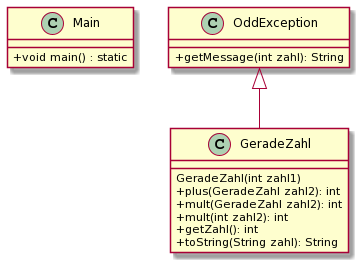
\includegraphics[scale=0.55]{uml/uml_c8_p1.png}

\subsection{Quelltext}
\subsubsection{Main.java}
\lstinputlisting[language = Java , frame = trBL , escapeinside={(*@}{@*)}]{../chapter_08/src/chapter_08/Main.java}
\subsubsection{GeradeZahl.java}
\lstinputlisting[language = Java , frame = trBL , escapeinside={(*@}{@*)}]{../chapter_08/src/chapter_08/GeradeZahl.java}
\subsubsection{OddException.java}
\lstinputlisting[language = Java , frame = trBL , escapeinside={(*@}{@*)}]{../chapter_08/src/chapter_08/OddException.java}

\subsection{Testdokumentation}
Bei einer Ungeraden Zahl wurde eine Exception geworfen und wie erwarte die Zahl
anschließend um eins erhöht.

\subsection{Benutzungshinweise}
Keine Besonderen Benutzungshinweise.
Das Programm muss lediglich nur ausgeführt werden.

\subsection{Anwendungsbeispiel}
\begin{lstlisting}[frame = trBL , escapeinside={(*@}{@*)}]
	[sebastian@laptop bin]$ java Main 	
	Error, 21 ist keine Gerade Zahl! Die Zahl wurde um Eins erhöht.
	Error, 13 ist keine Gerade Zahl! Die Zahl wurde um Eins erhöht.
	Zahl 1 = 220
	Zahl 2 = 22
	Zahl 3 = 660
	Zahl 4 = 24
	[sebastian@laptop bin]$ 
\end{lstlisting}